\section{System}
The system uses two arrays, each with three microphones. Three microphones along with a micro-controller are mounted at three vertices of an $20$cm equilateral triangle. Fig~\ref{fig:setup_array} shows a picture of the array. Micro-controller used in this project is \emph{teensy 3.1}. The micro-controller has $64$k RAM memory and the ADC is capable of sampling at $500$kHz. In this project, the micro-controller collects microphone data on all three channels for $12$ millisecond and then send the recorded data to a computer for localization. 

\begin{figure}[]
  \centering
  \begin{subfigure}[]{.2\textwidth}
    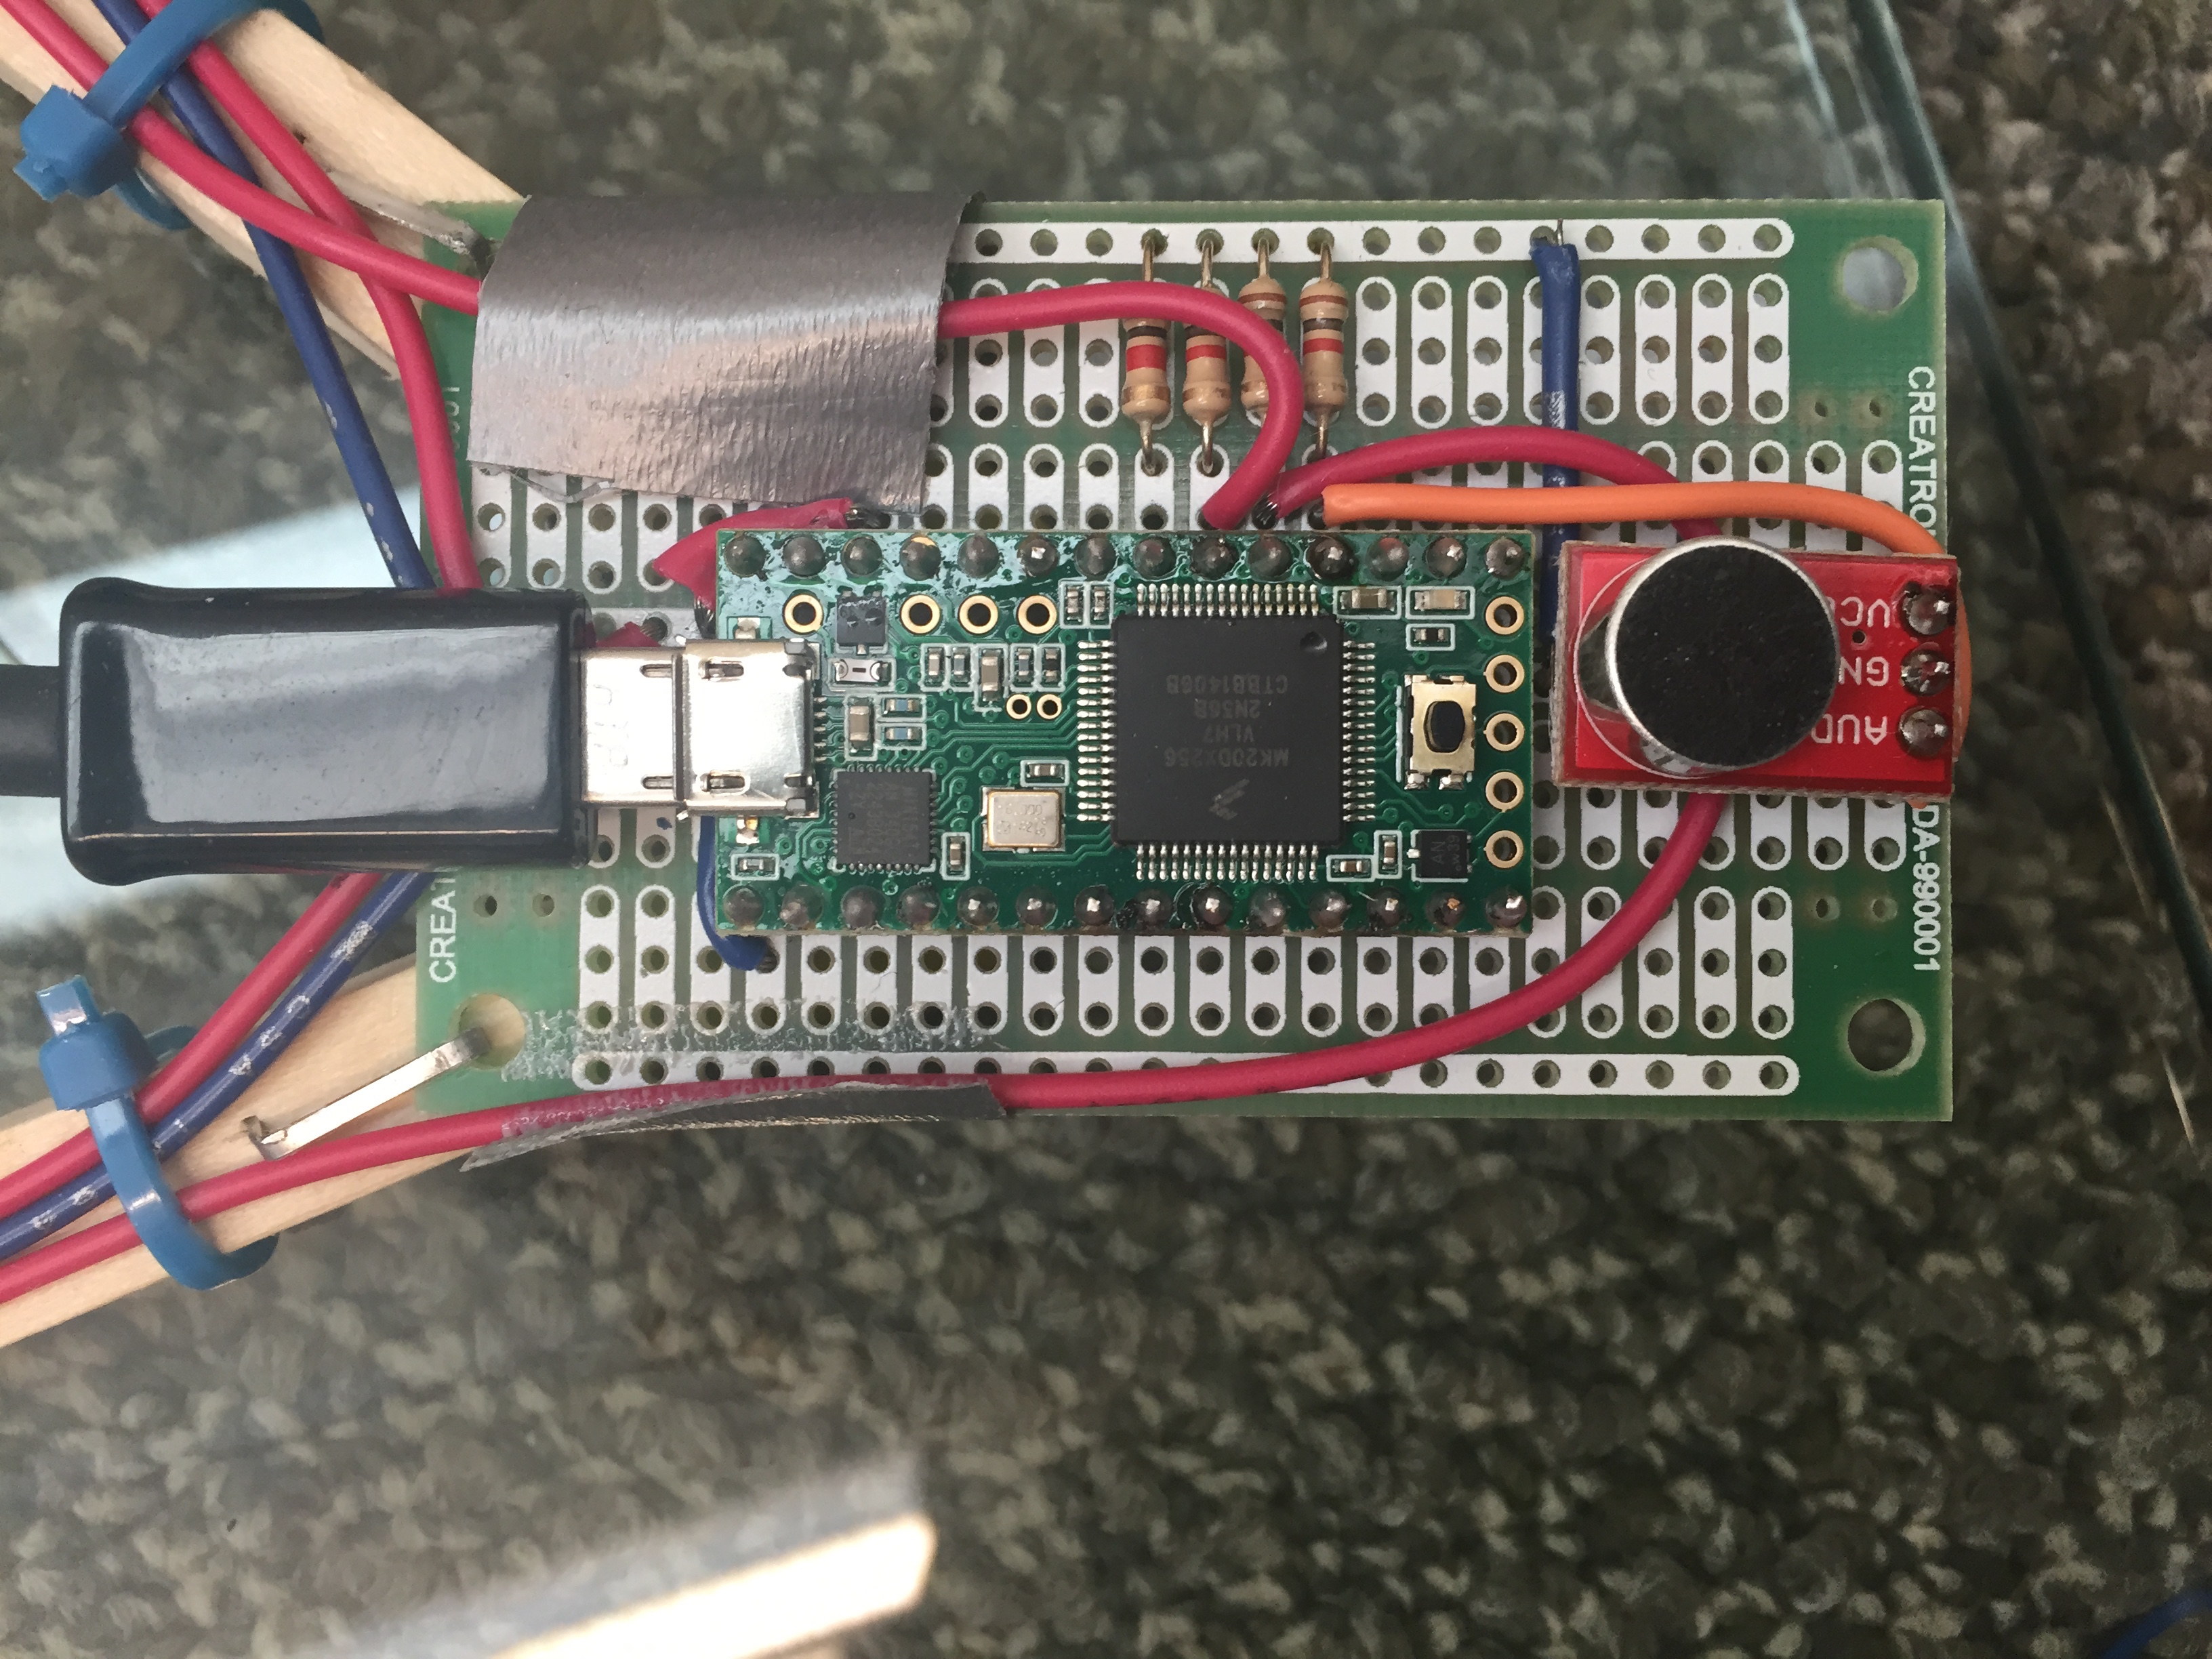
\includegraphics[width=\textwidth]{array_close.JPG}
  \end{subfigure}
  \begin{subfigure}[]{.2\textwidth}
    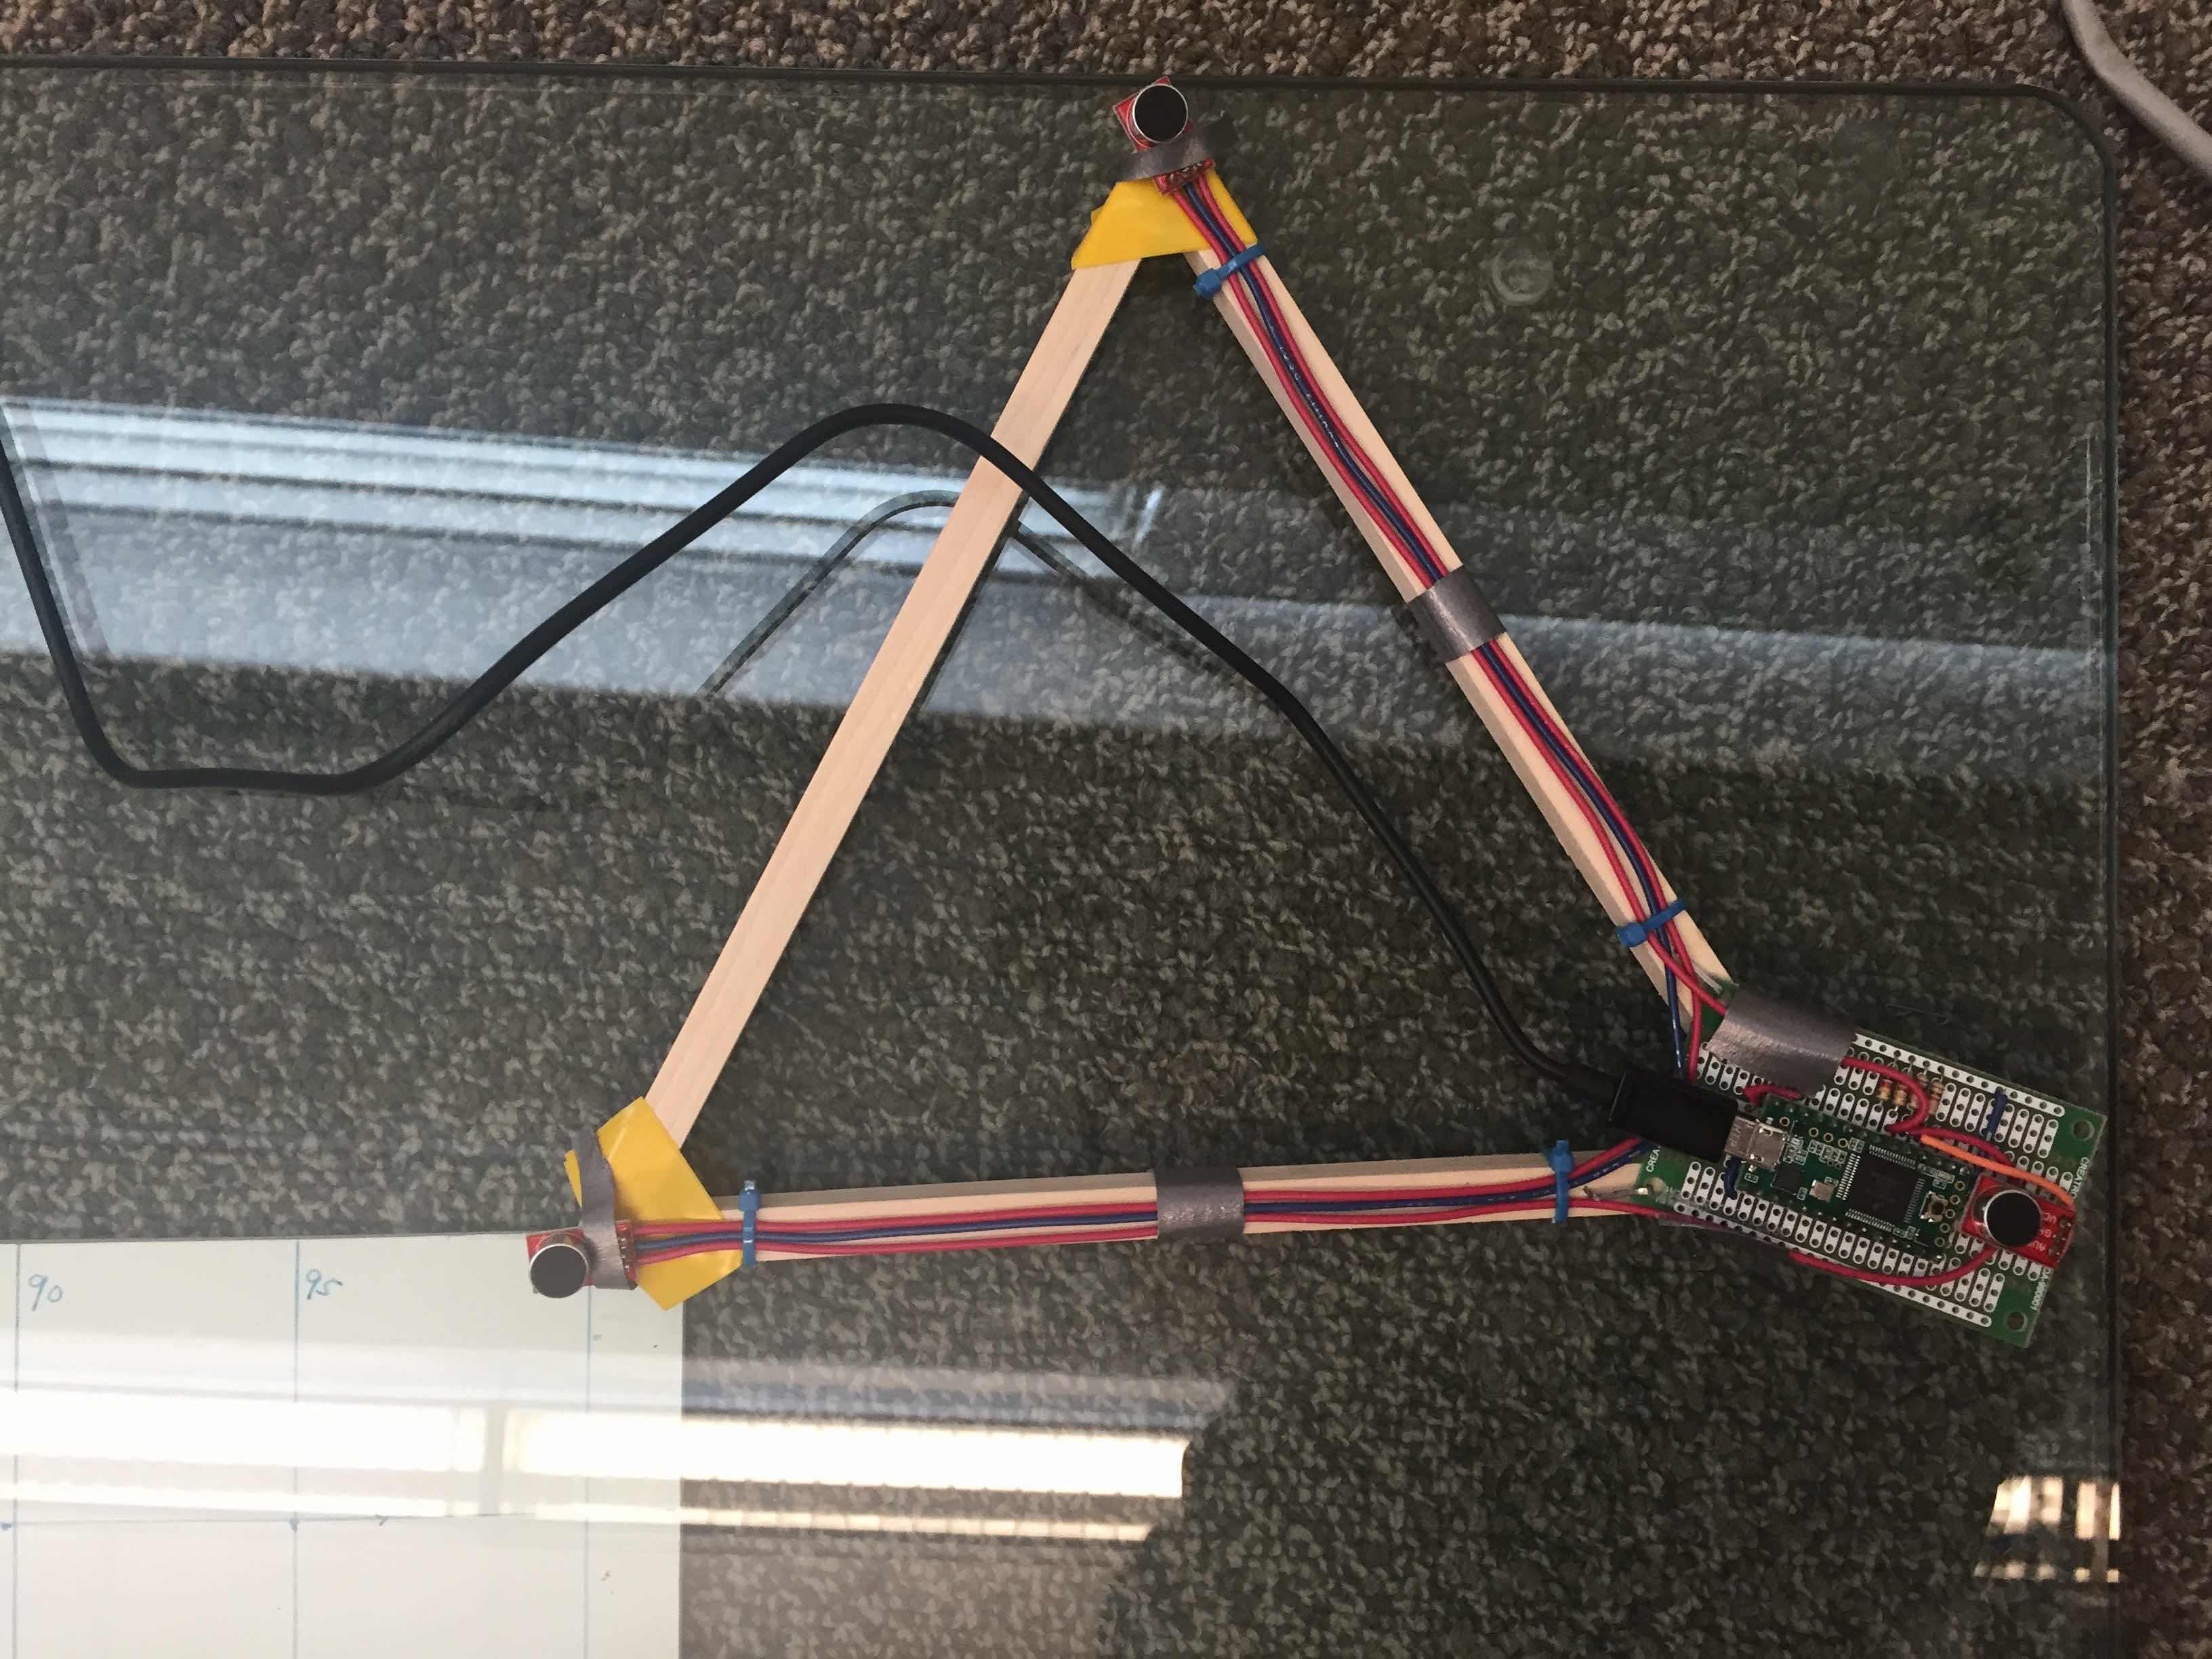
\includegraphics[width=\textwidth]{array.JPG}
  \end{subfigure}
  \caption{array}
  \label{fig:setup_array}
\end{figure}

To speed up computation for real time localization, instead of search for $t_0$ that maximizes equation~\ref{eq:gcc}. A grid-search in 2D grid is performed instead. With this approach, for each point in the grid, the arrival time difference to each microphone pair can be precomputed. Then localization resolves to calculating GCC for each microphone pair and performing a lookup for each point in the grid. To further improve localization accuracy, instead of using a point estimate for difference of arrival time, a liklihoood map is built. Each entry in GCC output is used as the liklihood for that delay. With three microphones $m_1,m_2,m_3$, for each location $(x,y)$ in the gird, the difference of arrival time to each microphones pair can be precomputed and stored in $D_{m_1,m_2}(x,y)$, $D_{m_1,m_3}(x,y)$, and $D_{m_2,m_3}(x,y)$. Let $R_{m_1,m_2}(\tau)$,$R_{m_1,m_2}(\tau)$, and $R_{m_1,m_2}(\tau)$ denote the GCC output for each microphone pair, then a liklihood map in the grid is calculated as:
\begin{eqnarray*}
  L(x,y) &=& R_{m_1,m_2}(D_{m_1,m_2}(x,y)) + R_{m_1,m_3}(D_{m_1,m_3}(x,y)) \\
 & & +R_{m_2,m_3}(D_{m_2,m_3}(x,y)) 
\end{eqnarray*}

Liklihood map from each array can be combined into final liklihood map:
\begin{equation}\label{eq:combine_l}
L(x,y) = L_1(x,y) L_2(x,y)
\end{equation}
, where $L_1(x,y)$ and $L_2(x,y)$ represents the liklihood map from array $1$ and array $2$

\begin{figure}[]
  \centering
  \begin{subfigure}[]{.15\textwidth}
    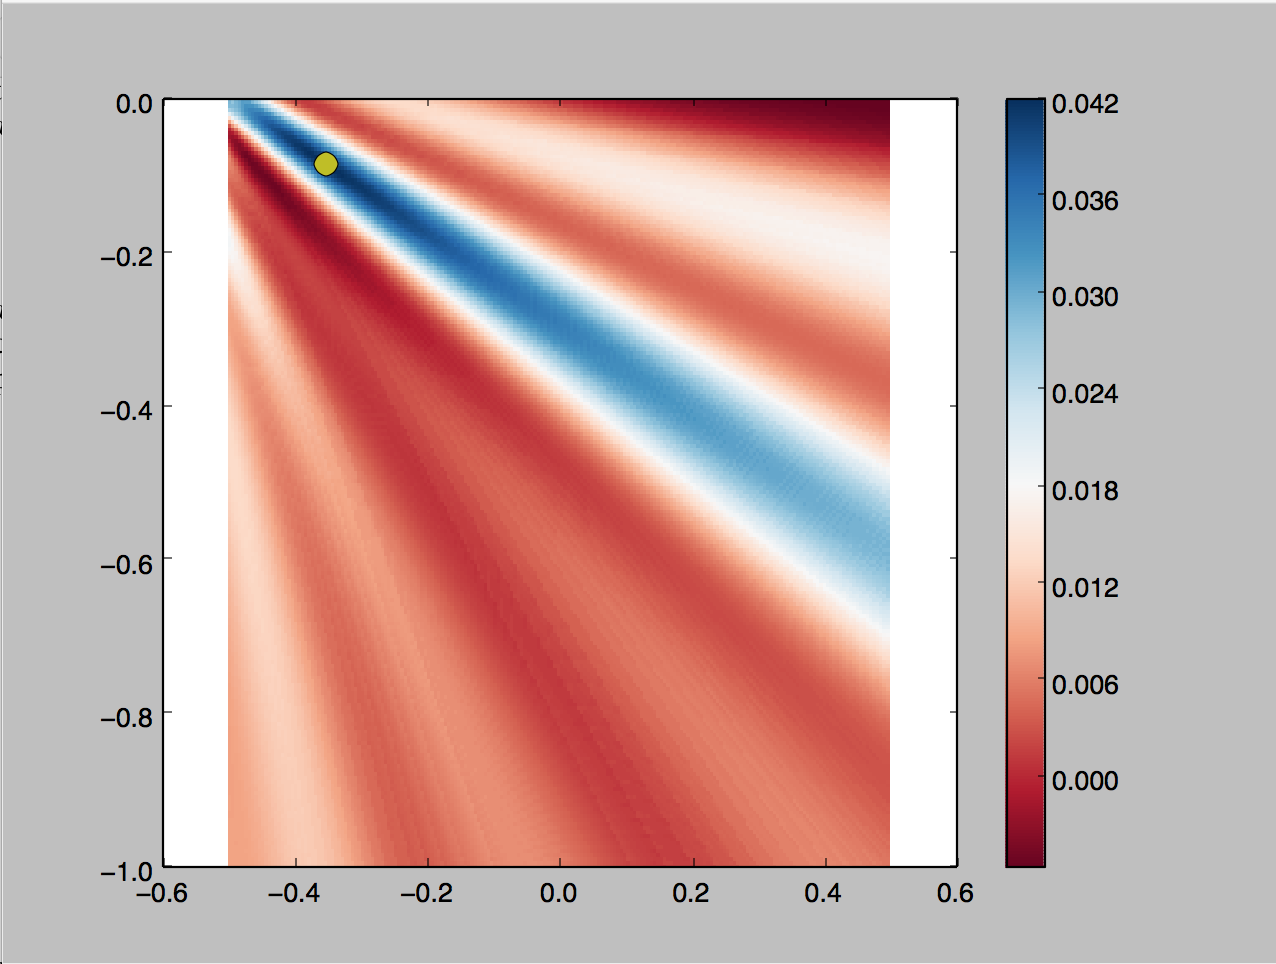
\includegraphics[width=\textwidth]{left.png}
    \caption{localization with only array 1}
  \end{subfigure}
  \begin{subfigure}[]{.15\textwidth}
    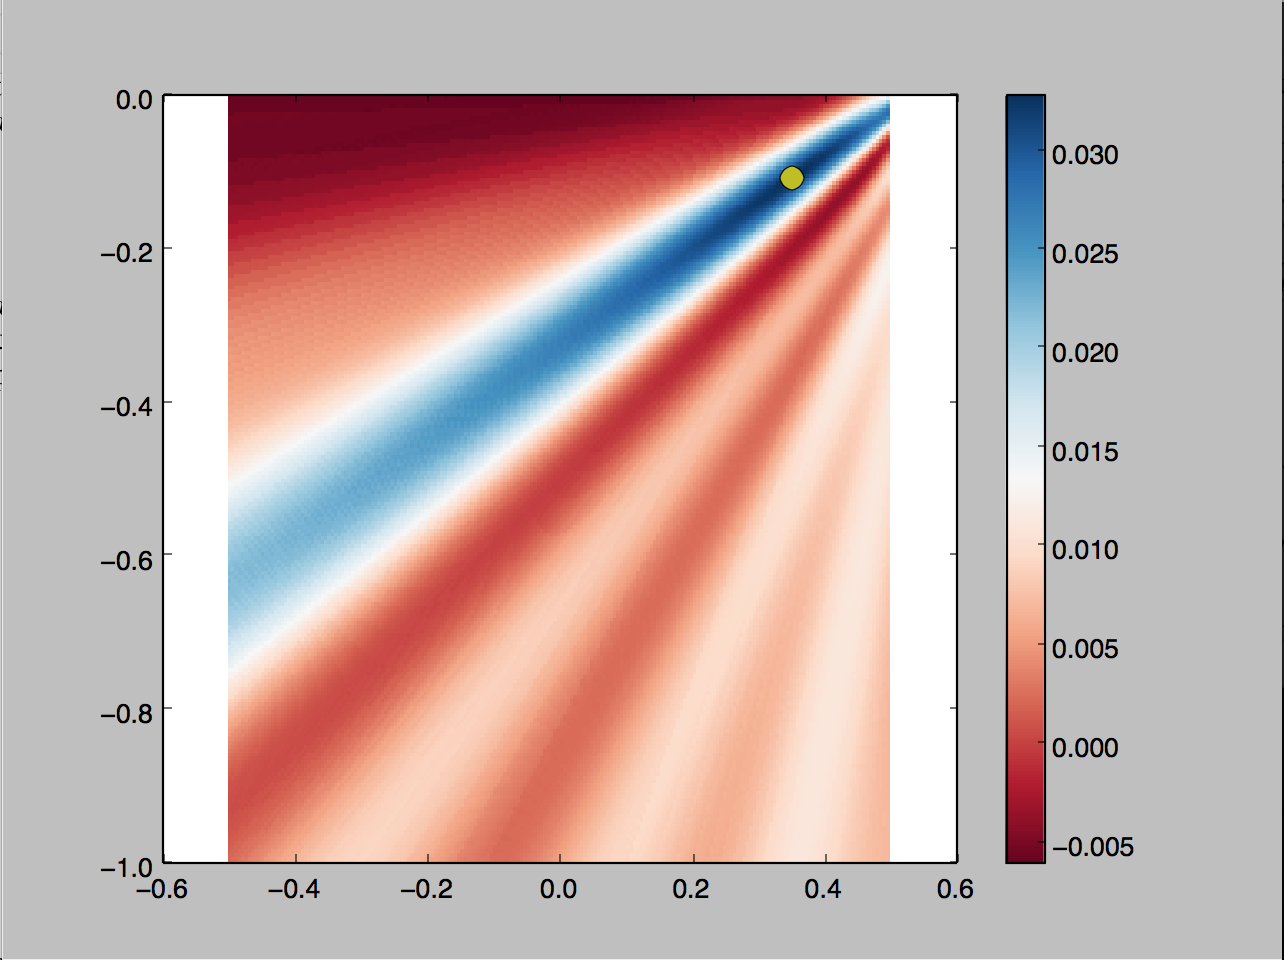
\includegraphics[width=\textwidth]{right.png}
    \caption{localization with only array 2}
  \end{subfigure}
  \begin{subfigure}[]{.15\textwidth}
    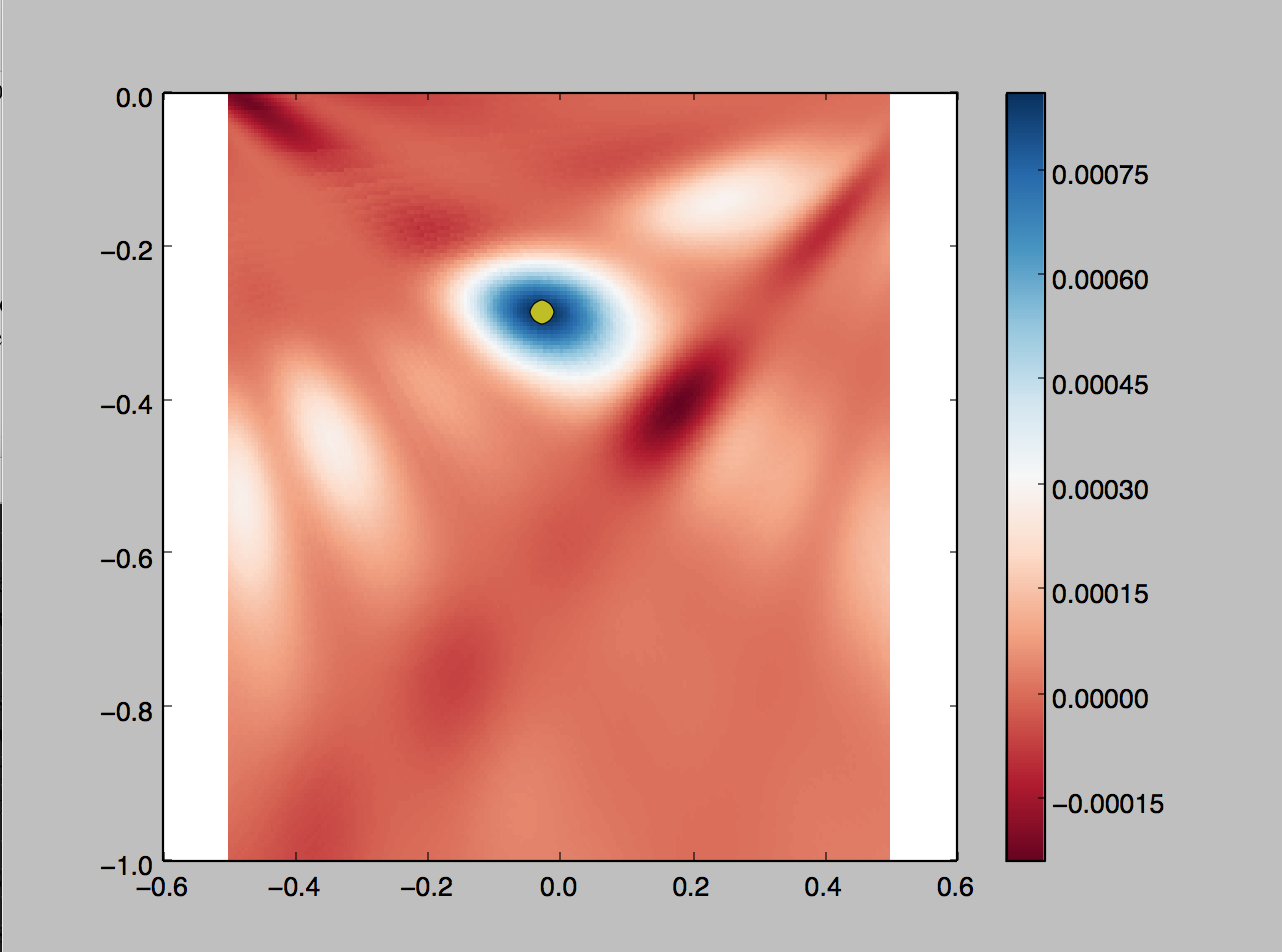
\includegraphics[width=\textwidth]{combined.png}
    \caption{localization with both arrays}
  \end{subfigure}
  \caption{Liklihood maps for localizating point at $(0.0,-0.3)$ m}
  \label{fig:liklihood}
\end{figure}


To see the effect of using multiple arrays, fig~\ref{fig:liklihood} shows the individual liklihood map from each array and also the combined liklihood according to equation~\ref{eq:combine_l}. Individual array gives accurate angle estimate, but has high uncertainty in distance estimate. By using two arrays, the angle estimate can be effectively combined to estimate distance.



From a timing point of view, the micro controller spends $12$ millisecond on sampling microphone data before sending the data to the computer for processing. Sending data through USB port takes another $18$ millisecond, and processing on computer takes around $50$ millisecond. Therefore, the totoal time lag between sound source and localization is around $80$ millisecond.
